\documentclass{sig-alternate}

\usepackage{url}
\usepackage{graphicx}

\newcommand{\nPrograms}{250,166}
\newcommand{\nAnalyzedPrograms}{247,798}
\newcommand{\nemptyPrograms}{14,307}
\newcommand{\nScriptPrograms}{233,491}
\newcommand{\nProgramsWithClones}{67,177}
\newcommand{\nLOC}{36,085,654}
\newcommand{\nscripts}{4,049,356}
\newcommand{\dup}{\emph{Duplication}~}

\newcommand{\todo}[1]{\textbf{#1}}

\begin{document}
%
% --- Author Metadata here ---
%\conferenceinfo{WOODSTOCK}{'97 El Paso, Texas USA}
% --- End of Author Metadata ---

\title{How Kids Code and How We Know:\\An Exploratory Study on the Scratch Repository }

\numberofauthors{1}
\author{
% 1st. author
\alignauthor
(anonymized submission)
%Ben Trovato\titlenote{Dr.~Trovato insisted his name be first.}\\
%       \affaddr{Institute for Clarity in Documentation}\\
%       \affaddr{1932 Wallamaloo Lane}\\
%       \affaddr{Wallamaloo, New Zealand}\\
%       \email{trovato@corporation.com}
% 2nd. author
%\alignauthor
%G.K.M. Tobin\titlenote{The secretary disavows
%any knowledge of this author's actions.}\\
%       \affaddr{Institute for Clarity in Documentation}\\
%       \affaddr{P.O. Box 1212}\\
%       \affaddr{Dublin, Ohio 43017-6221}\\
%       \email{webmaster@marysville-ohio.com}
}

%\date{30 July 1999}

\maketitle
\begin{abstract}
Block-based programming languages like Scratch, Alice and Blockly are becoming increasingly common as introductory languages in programming education. There is substantial research showing that those visual programming environments are suitable for teaching programming concepts. In this paper we explore the characteristics of Scratch programs. To that end we have scraped the Scratch public repository and retrieved 250.000 projects. We present an analysis of those projects in terms of complexity, used abstractions and programming concepts, and coding style. We found that programming abstraction concepts like functions are not commonly used. We further investigate the presence of code smells and bad programming practices, including code duplication, dead code, long method and large class smells. Our findings indicate that Scratch programs suffer from code smells and especially code duplication.
\end{abstract}

% A category with the (minimum) three required fields
%\category{H.4}{Information Systems Applications}{Miscellaneous}
%A category including the fourth, optional field follows...
%\category{D.2.8}{Software Engineering}{Metrics}[complexity measures, performance measures]

\terms{terms}

\keywords{Scratch, programming practices, code smells, static analysis}

\section{Introduction}

Scratch is a programming language developed to teach children programming by enabling them to create games and interactive animations. The public repository of Scratch programs contains over 12 million projects. Scratch is a \emph{block-based} language: users manipulate blocks to program. Block-based languages are visual languages, but also use some successful aspects of text-based languages such as limited text-entry and indentation, and as such are closer to `real', textual programming than other forms of visual programming, like dataflow languages are.

Block-based languages have existed since the eighties, but have recently found adoption as tools for programming education. In addition to Scratch, also Alice~\cite{conway_alice:_1994}, Blockly\footnote{\url{https://developers.google.com/blockly/}} and App Inventor~\cite{wolber_app_2011} are block-languages aimed at novice programmers.

refer to:
Research on the effectiveness of those languages for programming education
Research on programming habits
Our research on smells

The goal of this paper is to obtain a deep understanding of how people program in Scratch and to analyze the characteristics of Scratch programs. Moreover, knowing that bad programming habits and code smells can be harmful, we also want to explore whether they are common. Specifically, the research questions that we are trying to answer are:

\begin{itemize}
\item[RQ1] What are the size and complexity characteristics of Scratch programs?
\item[RQ2] Which coding abstractions and programming concepts and features are commonly used when programming in the Scratch environment?
\item[RQ3] How common are code smells and bad programming practices in Scratch programs?
\end{itemize}

Our study is based on data from the Scratch program repository. By scraping the list of recent programs \todo{link}, we have obtained \nPrograms~public Scratch programs and performed static analysis on them.

The contributions of this paper are as follows:

\begin{itemize}
	\item{A public data set of \nScriptPrograms~Scratch programs (Section \ref{dataset})}
	\item{An empirical evaluation of the data set for answering the aforementioned research questions}
\end{itemize}


\section{Background and Motivation}
\label{sec:background}
Block-based languages go back to 1986, when Glinert introduced the BLOX language~\cite{e._glinert_towards_1986}. BLOX consists of puzzle-like programming statements that can be combined into programs by combining them both vertically and horizontally. After a decade of little activity into block-based languages, they became a research topic again, starting with Alice~\cite{conway_alice:_1994}. More recently, new block-based languages have gained widespread popularity, especially powered by Scratch~\cite{resnick_scratch:_2009} and Blockly\footnote{\url{https://developers.google.com/blockly/}}. Over 100 million students have tried Blockly via Code.org, and the Scratch repository currently hosts over 12 million projects. Unlike in BLOX, in these new block-based languages the programming blocks can only be combined vertically, resembling textual code more.

Since their introduction, studies have demonstrated the applicability of block-based languages as a tool for education. Scratch, for example, was evaluated with a two-hour introductory programming curriculum for 46 subjects aged 14~\cite{meerbaum-salant_learning_2010}. This study indicated that Scratch could be used to teach computer science concepts: analysis of the pre- and post-tests showed a significant improvement after the Scratch course, although some concepts like variables and concurrency remained hard for students.

Moskal \emph{et al.}~\cite{b._moskal_evaluating_2005} compared computer science students who studied Alice before or during their first programming course to students that only took the introductory computer science course. Their results show that exposure to Alice significantly improved students' grades in the course, and their retention in computer science in general over a two year period. A follow-up study by Cooper \emph{et al.}~\cite{cooper_teaching_2003} obtained similar results, showing that a curriculum in Alice resulted in improved grades and higher retention in computer science.

Most convincingly, Price and Barnes performed a controlled experiment in which students were randomly assigned to either a text-based or a block-based interface in  which they had to perform small programming tasks~\cite{price_comparing_2015}. Their experiment showed that students in the block-based interface were more focused and completed more of the activity's goals in less time.

Summarizing the above, we conclude that block-based languages have a clear potential to be a great tool for introductory programming education, in some cases even outperforming text-based languages.

\subsection{Relevant Scratch Concepts}
\label{sec:scratch}
This paper is by no means an introduction into Scratch programming, we refer the reader to \cite{brennan_creative_2014} for an extensive overview. To make this paper self-contained, however, we explain a number of relevant concepts in this section. 

Scratch is a block-based programming language aimed at children, developed by MIT. Scratch can be used to create games and interactive animations, and is available both as a stand-alone application and as a web application. Figure \ref{fig:ui} shows the Scratch user interface in the Chrome browser.

\subsubsection{Sprites}
Scratch code is organized by `sprites': two-dimensional pictures each having their own associated code. Scratch allows users to bring their sprites to life in various ways, for example by moving them in the plane, having them say or think words or sentences via text balloons, but also by having them make sounds, grow, shrink and switch costumes. The Scratch program in Figure \ref{fig:ui} consists two one sprites, the cat, which is Scratch's default sprite and logo and a Piano. The code in Sprite1 will cause the cat to move right when the right arrow is pressed, and when the green flag is clicked it will continuously sense touching the piano.

\begin{figure}
	\begin{center}
		\includegraphics[width=\columnwidth]{fig/ui.png}
		\caption{The Scratch user interface consisting of the `cat' sprite on the left, the toolbox with available blocks in the category `Events' in the middle and the code associated with the sprite on the right. The upper right corner shows the actual location of the sprite.}
		\label{fig:ui}
	\end{center}
\end{figure} 

\begin{figure}
	\begin{center}
		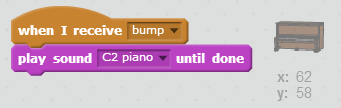
\includegraphics[width=2cm]{fig/bump.png}
		\caption{The script for the Piano sprite in Figure \ref{fig:ui}, causing a sound on receiving the `bump' signal.}
		\label{fig:bump}
	\end{center}
\end{figure} 

\subsubsection{Events}
Scratch is \emph{event-driven}: all motions, sounds and changes in the looks of sprites are initiated by events. The canonical event is the `when Green Flag clicked', activated by clicking the green flag at the top of the user interface. In addition to the green flag, there are a number of other events possible, including key presses, mouse clicks and input from a computer's microphone or webcam. The Scratch code in Sprite1 in Figure \ref{fig:ui} contains two events: `when Green Flag clicked' and `when right arrow key pressed', each with associated blocks.

\subsubsection{Signals}
Events within Scratch can be user generated too: users can broadcast a message, for example when two sprites touch each other, like in Figure \ref{fig:ui}. All other sprites can then react by using the `when I receive' Hat block. In Figure \ref{fig:ui}, Sprite1 broadcasts `bump' when the cat touches the Piano. The Piano reacts on that by making a sound, see Figure \ref{fig:bump}.

\subsubsection{Scripts}
Source code within sprites is organized in scripts: a script can start with an event (a Hat block\footnote{\url{http://wiki.scratch.mit.edu/wiki/Hat_Block}}) which indicates when something should happen. A hat block can be followed by an arbitrary number of other blocks. 

The Scratch code in Figure \ref{fig:ui} has two distinct scripts, one started by clicking on the green flag and one by pressing the space bar. It is possible for a single sprite to have multiple scripts initiated by the same event. In that case, all scripts will be executed simultaneously.

\subsubsection{Procedures}
Scratch users can define their own blocks, with a pop-up screen displayed in on the left hand side of Figure \ref{fig:twoBlocks}. As shown in this Figure, Scratch users can set the name of the sprite and define input parameters. The block in Figure \ref{fig:twoBlocks} uses two parameter, one textual (string1) and one numerical (number1). A user-created block is programmed using ordinary Scratch blocks as shown on the right hand side of Figure \ref{fig:twoBlocks}.

\subsubsection{Remixing}
\todo{maybe only useful with we will talk about remixing in the remainder?}
Scratch programs can be shared by their creators in the global Scratch repository\footnote{\url{https://scratch.mit.edu/explore/projects/all/}}. Shared Scratch programs can be `remixed' by other Scratch users, which means that a copy of this program is placed in the user's own project collection, and can be then further changed. The `remix tree' of projects is public, so users can track which users remix their programs, a bit similar forking in GitHub. Contrary to forking though, changes upstream cannot be integrated back into the original project.

\begin{figure}
	\begin{center}
		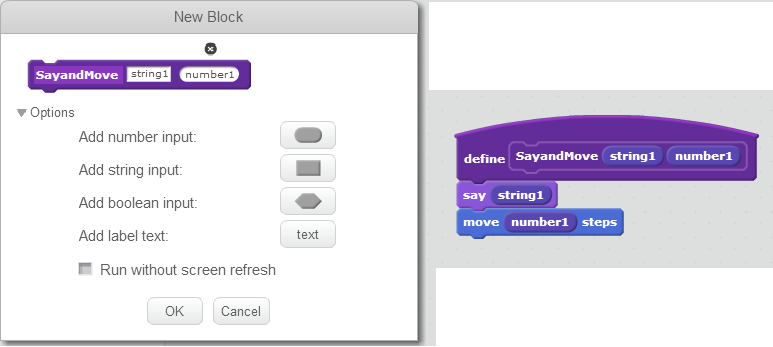
\includegraphics[width=8cm]{fig/twoBlocks.png}
		\caption{The user interface for creating and defining user-defined blocks \todo{could be nicer}}
		\label{fig:twoBlocks}
	\end{center}
\end{figure} 



\section{Research design and dataset}
\label{researchDesign}

The main focus of this study is to understand how people program in Scratch by analyzing the characteristics of Scratch programs. To answer our research questions, we conducted an empirical quantitative evaluation of program data we collected from the Scratch repository. The dataset is described in Section \ref{dataset}. \todo{Below, we present how we approached each research question.}

\textbf{RQ1} What are the size and complexity characteristics of Scratch programs? quantitative analysis, provide and analyze descriptive statistics on the size, complexity metrics, statistical analysis . mentioned taht it was imported to db and done and statistical data from db queries? The outcomes are presented in Section...

\textbf{RQ2} Which coding abstractions and programming concepts and features are commonly used when programming in the Scratch environment? Using the code in the dataset, we perform a detailed statistical analysis of code characteristics to answer RQ2 (Section ??). We manually assigned types to commands/blocks.

\textbf{RQ3} Which code smells and bad programming practices are common in Scratch programs?  to examine if coding style conventions are used, we qualitatively analyze..

\subsection{Dataset}
\label{dataset}
\subsubsection{Obtaining Scratch programs}
We obtained the set of Scratch programs by using a scraping program. Our scraping program called Kragle starts by reading \url{https://scratch.mit.edu/explore/projects/all/} and thus obtaining program ids of programs that were most recently shared. Subsequently, Kragle obtains the JSON code for each of the listed programs. In addition to the programs themselves, Kragle also gathers metadata including the numbers of views, loves, favorites and remixes.

 % For a given id $x$ a Scratch programs JSON representation can be obtained via \url{https://cdn.projects.scratch.mit.edu/internalapi/project/x/get}.  Does not fit on the page nicely and might also not be needed?

We ran Kragle on March 2nd 2016 and let it running for 24 hours, when it had obtained a little over 250.000 programs.  Out of the \nPrograms~, we failed to parse and further analyze 2.367 programs due technical difficulties with the provided JSON files. Kragle, as well as all scraped programs and our analysis files are available\footnote{\url{https://github.com/ScratchLover42/ICER-Data-Code}}.

\subsubsection{Analyzing the Scratch programs}
Once we obtained the Scratch programs, we parsed the JSON files according to the specification of the format\footnote{\url{http://wiki.scratch.mit.edu/wiki/Scratch_File_Format_(2.0)}}. This resulted in a list if used blocks per program, with the sprites and the stage of the program. We also assign types to all the blocks, both their shapes and the tab they originate from. For example, When Green Flag Clicked is a \emph{Hat block} from the \emph{Events category}.


\section{Results}

In the following sections we describe the results obtained for each of the research questions through the analysis of the \nAnalyzedPrograms~Scratch projects in our dataset.

\subsection{Program size and complexity}

The dataset is found to contain a relatively small number of projects without any code: \nemptyPrograms (5.77\%). Through random manual sampling we found that in some cases those projects contained sprites and costumes but no code and in others they were entirety empty apart from the Scratch cat added by default. Since those projects are empty in terms of code we excluded them from further analysis, leaving the final number of analyzed non-empty projects to \nScriptPrograms.

\begin{table*}[ht]
	\centering
	\begin{tabular}{lrrrrrr}
		\hline
		&\textbf{mean}&\textbf{min}&\textbf{Q1}&\textbf{median}&\textbf{Q3}&\textbf{max}\\
		\hline
		Sprites with code per project&5.68&1&1&2&5&525\\
		Scripts per project&17.35&1&2&5&12&3038\\
		Maximum indentation per project&4.56&1&3&3&5&488\\
		Lines of code (LOC) per project&154.55&1&12&29&76&34622\\
		LOC in Stage per project&4.80&0&0&0&3&2613\\
		LOC in Sprites per project&115.57&0&10&26&68&34613\\
		LOC in Procedures per project&34.17&0&0&0&0&20552\\
		McCabe Cyclomatic Complexity (CC) per script&1.58&1&1&1&1&246\\
		McCabe CC per procedure script&3.75&1&1&2&4&183\\
		Procedures per project with procedures&11.50&1&1&2&6&847\\
		Arguments per Procedure&0.95&0&0&0&1&53\\
		Numerical arguments per procedure with arguments&1.73&0&1&1&2&22\\
		Text arguments per procedure with arguments&0.28&0&0&0&1&24\\
		Boolean arguments per procedure with arguments&0.13&0&0&0&0&14\\
		Calls per procedure&2.14&0&1&1&2&526\\
		Scripts with calls per procedure&1.13&0&1&1&1&59\\
		Variables per project&2.06&0&0&0&1&340\\
		Scripts utilizing variable&4.97&1&1&3&5&1127\\
		Lists per project&0.55&0&0&0&0&319\\
		Conditional statements per project&10.02&0&0&0&3&5950\\
		Recursive loop statements per project&7.65&0&1&2&5&2503\\
		Broadcast-receive statements per project&8.57&0&0&0&2&2460\\	
		\hline
	\end{tabular}
	\caption{Summary statistics from the dataset of \nScriptPrograms~non-empty Scratch projects}
	\label{tbl-size}
\end{table*}

\begin{table*}[ht]
	\centering
	\begin{tabular}{lrr}
		\hline
		&\textbf{number}&\textbf{percentage}\\
		\hline
		Retrieved projects & 250,166 & \\
		Analyzed projects & 247,798 & \\
		Non-empty projects (used for statistics) & \textbf{233,491} & \\

		Projects utilizing variables & 73,577 & 31.51\% \\
		Projects utilizing lists & 9,358 & 4.01\% \\
		Projects with conditional statements & 92,959 & 39.81\% \\
		Projects with recursive loop statements & 180,210 & 77.18\% \\
		Projects with \texttt{repeat until <condition>} statements & 31,739 & 13.59\% \\
		Projects with \texttt{broadcast} - \texttt{receive} statements & 69,039 & 29.57\%\\
		Projects with cloned scripts (>=5 blocks) across sprites & 59,634 & 25.54\% \\
		Projects with cloned scripts (>=5 blocks) within sprites & 23,671 & 10.14\%\\
		Projects with cloned procedures (>=5 blocks) & 4,945 & 2.12\%\\
		Projects with cloned functionality blocks (>=4 blocks) across sprites & 60,554 & 25.93\%\\
		Projects with exact clones (>=5 blocks) across sprites & 27,574 & 11.81\%\\
		Projects with exact clones (>=5 blocks) within sprites & 2,043 & 0.87\%\\
		\hline
	\end{tabular}
	\caption{Characteristics in the projects in the dataset}
	\label{tbl-characteristics}
\end{table*}

\begin{figure}
	\centering
	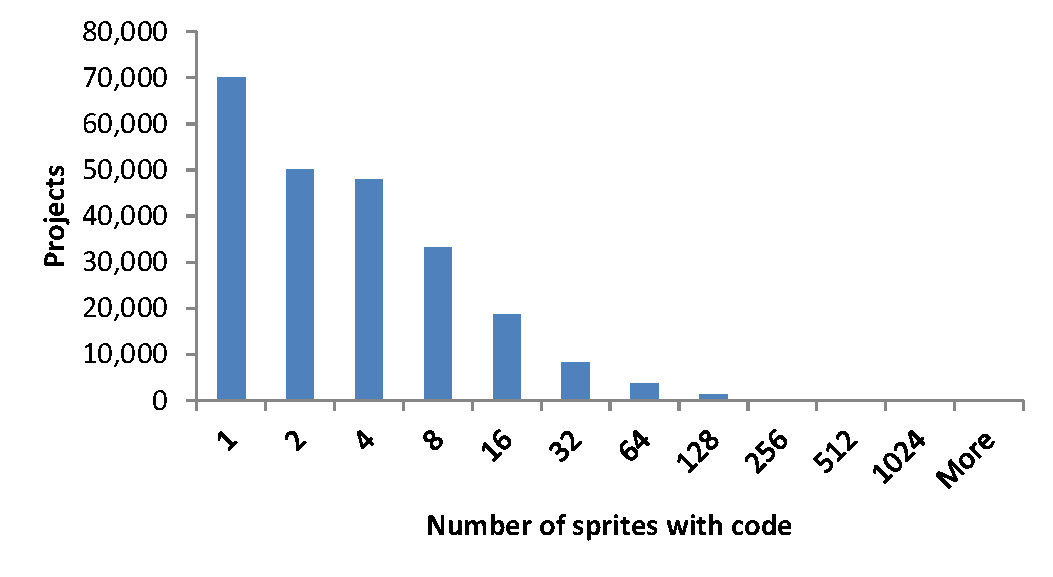
\includegraphics[width=0.45\textwidth]{fig/charts/1sprites}
	\caption{Histogram of the number of sprites in the analyzed projects}
	\label{fig:size-sprites}
\end{figure}
\begin{figure}
	\centering
	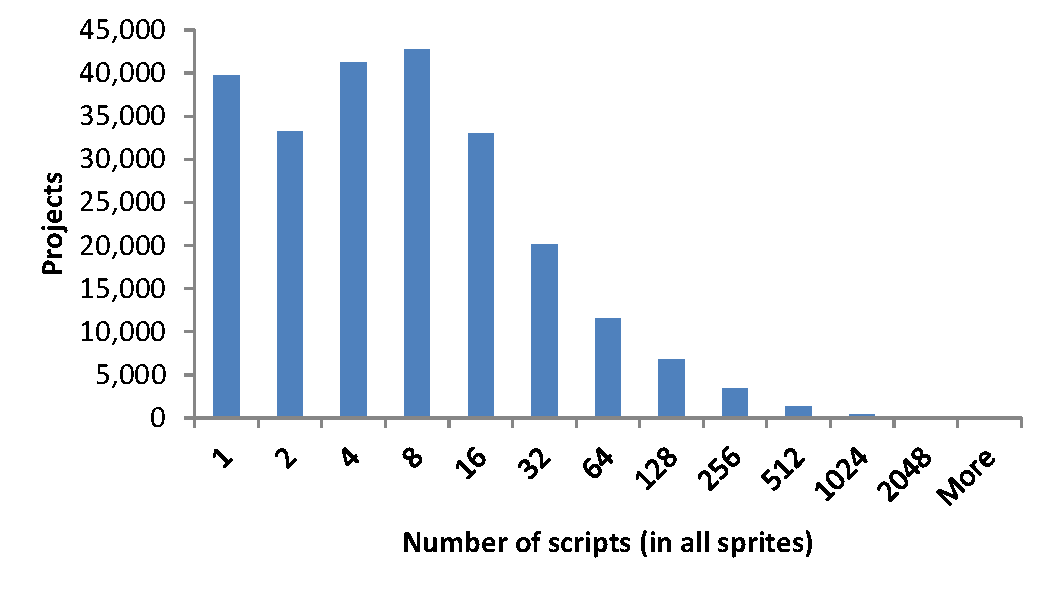
\includegraphics[width=0.45\textwidth]{fig/charts/1scripts}
	\caption{Histogram of the number of scripts in the analyzed projects}
	\label{fig:size-scripts}
\end{figure}
\begin{figure}
	\centering
	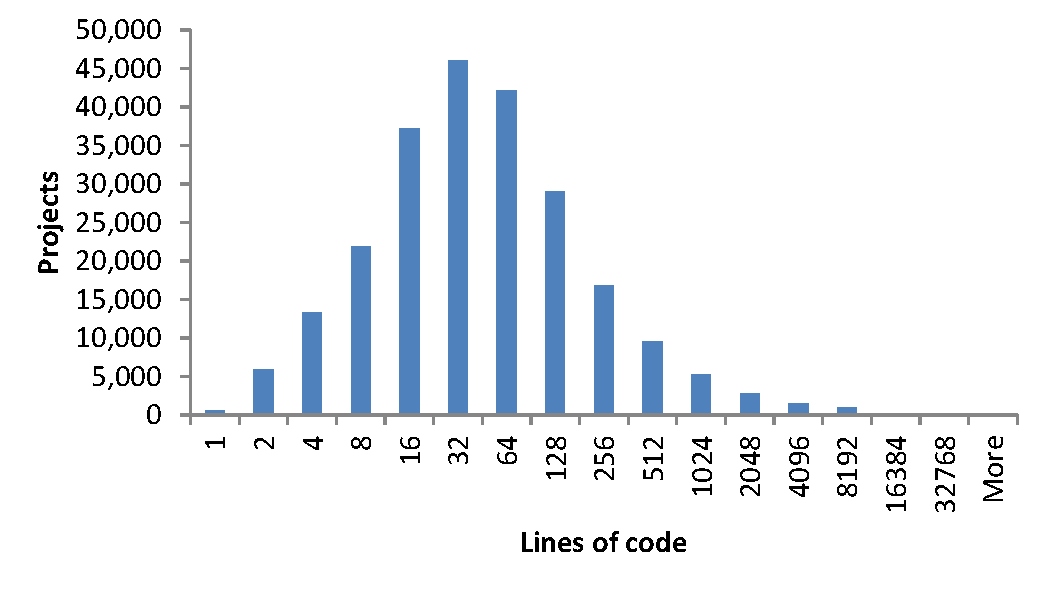
\includegraphics[width=0.45\textwidth]{fig/charts/1locs}
	\caption{Histogram of the lines of code in the analyzed projects}
	\label{fig:size-locs}
\end{figure}
\begin{figure}
	\centering
	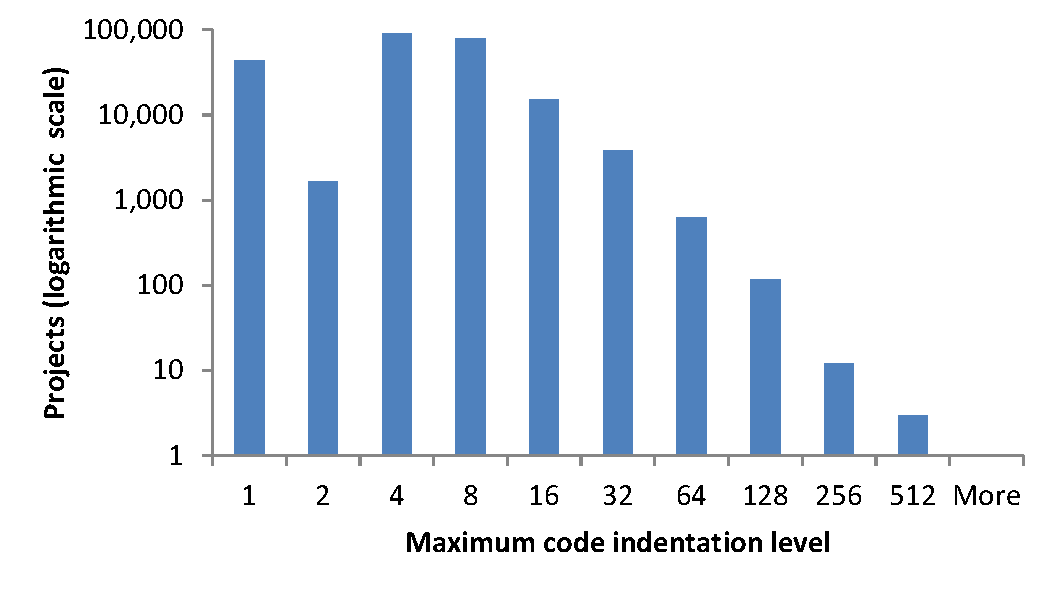
\includegraphics[width=0.45\textwidth]{fig/charts/1indent}
	\caption{Histogram of the maximum code indentation level in the analyzed projects}
	\label{fig:size-indent}
\end{figure}
\begin{figure}
	\centering
	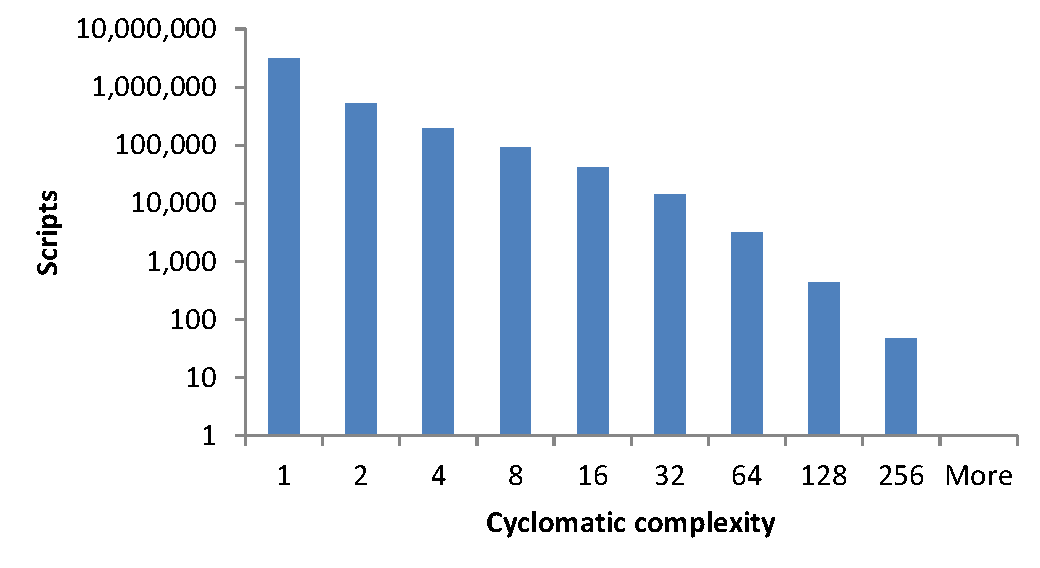
\includegraphics[width=0.45\textwidth]{fig/charts/3cyclomatic}
	\caption{Histogram of the McCabe cyclomatic complexity of the \nscripts~analyzed scripts}
	\label{fig:cyclomatic}
\end{figure}


In Table \ref{tbl-size} we summarize statistics for metrics related to size and complexity. We use the mean value and the five-number summary to describe the dataset in terms of the number of sprites with code per project (including the stage sprite) and the number of scripts per project, where each script is a code-block of interconnected Scratch blocks. For example, in Figure \ref{fig:ui} the cat sprite contains two scripts. We further measure the lines of code per project, considering each Scratch block to represent exactly one line of code, thus not counting the closing constructs of loops or conditional statements as separate lines. Furthermore, we measure the nestedness of program, which is the number of times blocks are placed within each other. For example, the program in Figure \ref{fig:ui} has a maximum indentation of 3 in the `Wgen Green flag clicked' script, as that has a broadcast block within an if, within a forever\todo{for Felienne: double check}. Figures \ref{fig:size-sprites}, \ref{fig:size-scripts}, \ref{fig:size-locs} and \ref{fig:size-indent} plot the distribution of those size metrics.

We find that the majority of Scratch projects are small; 75\% of the projects have up to 5 sprites, 12 scripts and 76 lines of code, while one fourth of the projects have up to 12 lines of code. On the other end, 5\% of the projects (11,712) are found to have more than 18 sprites and 4.8\% (11,214) consist of more than 500 lines of code. The analysis also highlighted some surprisingly large projects: 135 with more than 300 sprites and even 30 projects with more than 20,000 lines of code\footnote{The Scratch identifiers of those projects can be found in \todo{link}}.

The lines of code metric was further analyzed to understand code organization. As shown in Table \ref{tbl-size}, the majority of Scratch code---74.78\% out of \nLOC~lines of code---is written within sprites. An additional 3.1\% of the total lines are found in the stage class. More interestingly, the remaining 22.11\% are lines within defined procedures, which are found in only 7.7\% (17,979) of the projects. Those projects that contain procedures use them a lot; almost half of their total lines of code (48.81\%) are lines within procedures.

As a complexity metric we also used the McCabe cyclomatic complexity \cite{mcCabe76},  a quantitative measure of the number of linearly independent paths through a program's source code. This is calculated per script by counting the number of decision points in the script plus one. In Scratch, decision points can be the \texttt{if} and \texttt{if else} blocks. The results of the cyclomatic complexity metric per script are plotted in Figure \ref{fig:cyclomatic}. The majority (78.33\%) of \nscripts scripts contain no decision points, while 13.08\% have a cyclomatic complexity of 2, containing exactly one decision point. The complexity is higher, over 4, for 3.67\% of the scripts. The analysis also highlighted 209 scripts with a cyclomatic complexity over 100 and up to 246\footnote{The Scratch identifiers of those projects can be found in \todo{link}}. Cyclomatic complexity was greater (mean value of 3.32\%) in defined procedures, with 56.46\% of the procedures having at least one decision point.

\noindent
\fbox{
	\begin{minipage}{0.46\textwidth}
		RQ1: The majority of Scratch projects are small and simple; 75\% of the projects have up to 5 sprites, 12 scripts, 76 lines of code and no decision points. Most code is written in sprites. A small number of projects (7.7\%) use procedures, but they use them a lot and for more complex code. There exist surprisingly large and complex projects.
	\end{minipage}}

\subsection{Programming abstractions and concepts}

The first method for abstraction that we investigate is the use of procedures. In the dataset we found 206,799 procedures in 17,979 projects. As summarized in Table \ref{tbl-size}, the projects that contain procedures have an average of 11.5 procedures, but with 53.59\% of those projects having up to 2. Figure \ref{fig:proceduresperproject} shows the distribution of procedures in projects. Regarding procedure arguments, we found that 55.57\% have no arguments and 19.48\%\% have only one (shown in Figure \ref{fig:procedurearguments}). The majority of procedure arguments (80.59\%) are numeric, and the least used argument type is the boolean one---6.23\% of the total procedure arguments, found in 5.32\% of the procedures.

\begin{figure}
	\centering
	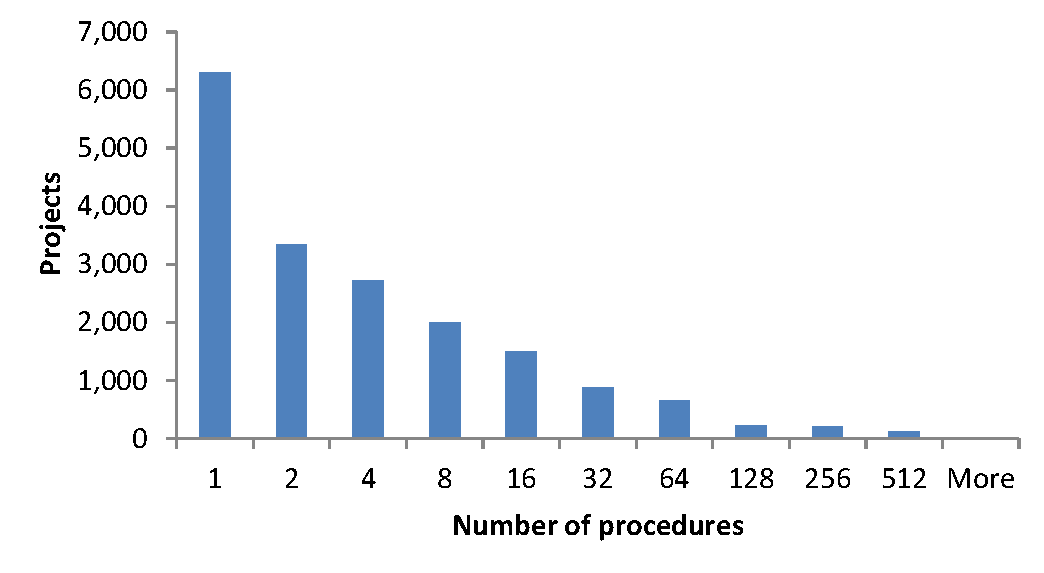
\includegraphics[width=0.45\textwidth]{fig/charts/6proceduresperproject}
	\caption{Histogram of the number of procedures for the 17,979 projects that include at least one}
	\label{fig:proceduresperproject}
\end{figure}

\begin{figure}
	\centering
	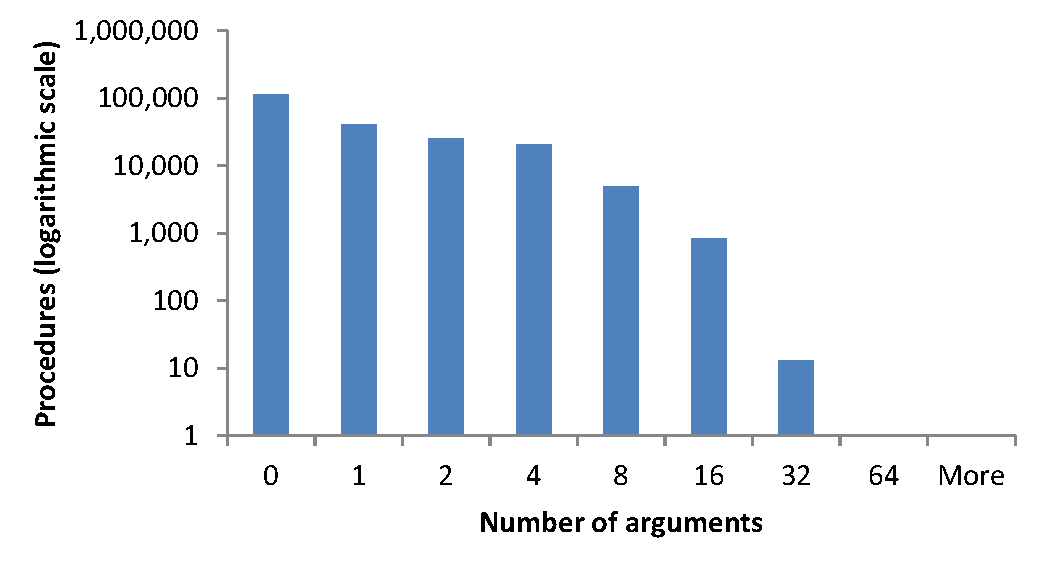
\includegraphics[width=0.45\textwidth]{fig/charts/5arguments}
	\caption{Histogram of the number of arguments for the procedures in the dataset}
	\label{fig:procedurearguments}
\end{figure}

The use of procedures in projects was further investigated through the procedure calls, summarized in Figure \ref{fig:procedurecalls}. A significant number of the defined procedures (13,036 or 6.3\%) are not called in the projects. Most procedures are called exactly once (62.32\% of them) or twice (15.65\% ) and from exactly one script (85.92\% of them). Examining the origin of procedure calls, we found remarkable that most of the calls (56.09\%) originate from other procedures, and even 1.06\% originate from the same procedure, thus making it recursive. Those recursive procedures are found in 1052 projects.\footnote{list of recursive procedures published \todo{link}}.

\begin{figure}
	\centering
	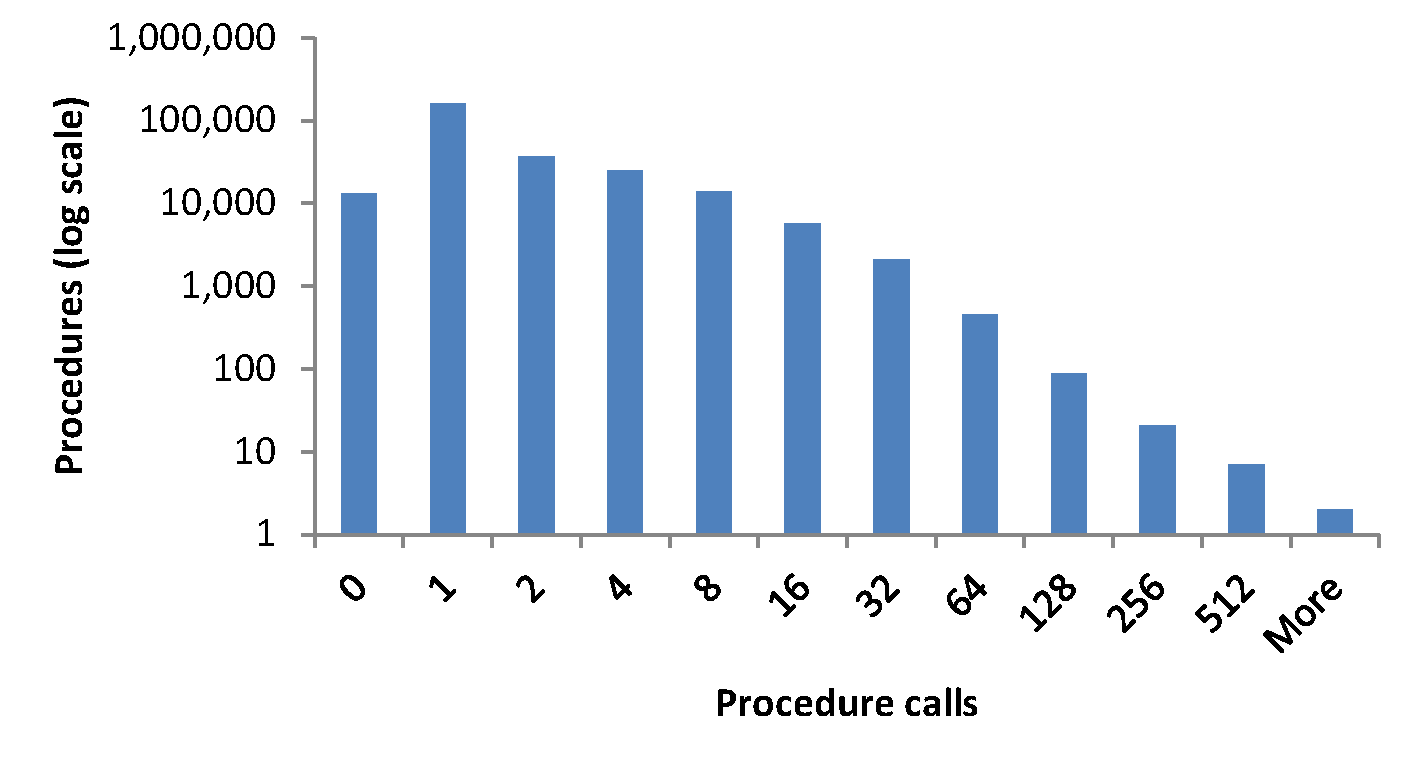
\includegraphics[width=0.45\textwidth]{fig/charts/7procedurecalls}
	\caption{Histogram of the number of calls of each procedure in the dataset}
	\label{fig:procedurecalls}
\end{figure}

As shown in table \ref{tbl-characteristics}, almost one-third of the projects utilize variables and a small number (4.01\%) utilize lists. The number of variables that is being used is also limited, with only 7.48\% of the projects having 5 or more variables. The distribution of variable and list utilization is shown in Figure \ref{fig:variables}. Exceptional cases exist: the analysis highlighted 842 projects with more than 100 variables and up to 340. Examining the initialization of variables through the \texttt{set <variable> to <value>} blocks, we found that for 4.83\% of all variables this was missing. The scope of variables was also analyzed: As shown in Table \ref{tbl-size}, each variable is used by an average of 4.97 different scripts, with a median value of 3. However, we must note that this measurement might not be entirely accurate, because variables might be defined in the scope of specific sprites. With our dataset we cannot differentiate global from local variables and we would consider local variables defined with the same name in different sprites as global variables.

\begin{figure}
	\centering
	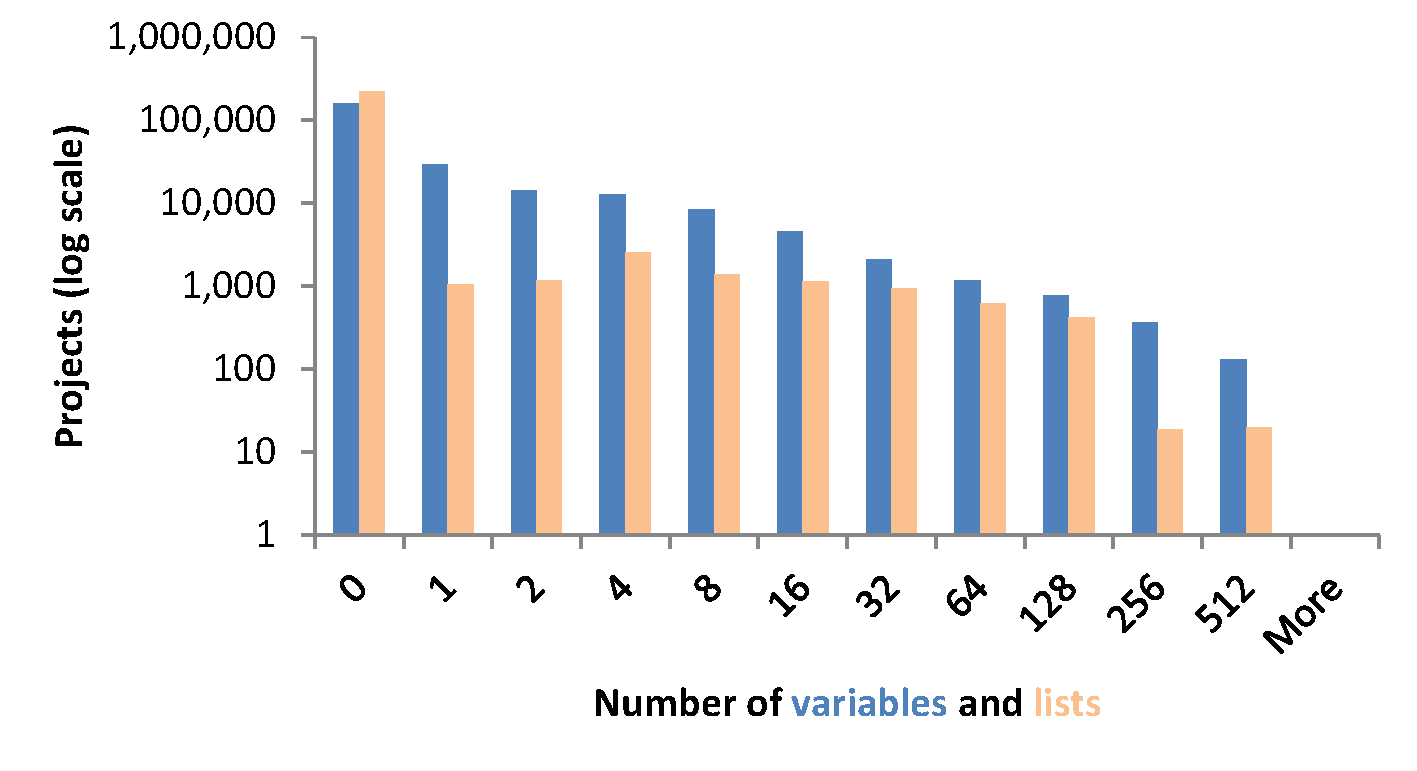
\includegraphics[width=0.45\textwidth]{fig/charts/8variableslists}
	\caption{Histogram of the number of variables and lists utilized in the projects}
	\label{fig:variables}
\end{figure}

Regarding program control features, conditional statements (blocks \texttt{if <condition> then} and \texttt{if <condition> then else}) are used by 39.81\% of the projects. Recursive loops (blocks \texttt{repeat <times>}, \texttt{forever} and \texttt{repeat until <condition>}) are more common, used by 77.18\% of the projects. The most common of the three is the \texttt{forever} block, accounting for 51.86\% of all recursive loops and the least common one is the \texttt{repeat until <condition>} block, accounting for 11.57\% and used in 13.59\% of the total projects.
	
For event management Scratch offers blocks \texttt{broadcast}, \texttt{broadcast and wait} and \texttt{when I receive}. 
Those blocks are utilized by 29.57\% of the projects. \texttt{broadcast and wait} is rarely used, in only 3.87\% of the projects. The events are not always synchronized: 3,33\% of the \texttt{when I receive} blocks were found to wait for a message that is never being broadcasted, while 4,4\% of the \texttt{broadcast} blocks broadcast a message that is not being received. This lack of syncronizations occurs in 18,669 projects (7.99\% of the total non-empty ones).

%user interativity		
\noindent
\fbox{
	\begin{minipage}{0.46\textwidth}
RQ2: One third of the projects utilize variables, sometimes without initializing them. 39.81\% of the projects utilize conditional statements and 77.18\% recursive loops, but conditional recursion is rarely used. 29.57\% of the projects utilize broadcast and receive blocks, but in 29.57\% of the projects they are not synchronized. Most procedures are called once or twice, from a single script which, in more than half of the cases, is another procedure. Recursive procedure calls exist in 1052 (0.45\% of the total) projects.
	\end{minipage}
	}

\subsection{Code smells and bad programming practices}

The duplicated code smell is the first smell that we examine. The first step for our analysis is to specify what we consider a code clone in the context of Scratch programming: a script that is composed of a set of blocks of the same type connected in the same way and is repeated within or across sprites of the same program. For the identification of clones we do not take into account the values of the parameters that may be used in the blocks, so that two blocks that only differ in the values of parameters are considered to be equal. We also examined the case of clones with the same parameter values, and we refer to them as \textit{exact clones}. The next step in the analysis is to determine the minimum size of the scripts that are considered clones instead of incidentally similar. For this, we examine the number of detected clones for different script sizes and present the results in Figure \ref{fig:cloneslines}. Based on this distribution, we opt to adopt the number also used by the authors in \cite{moreno_automatic_2014}, which is the minimum size of 5 blocks per script.

\begin{figure}
	\centering
	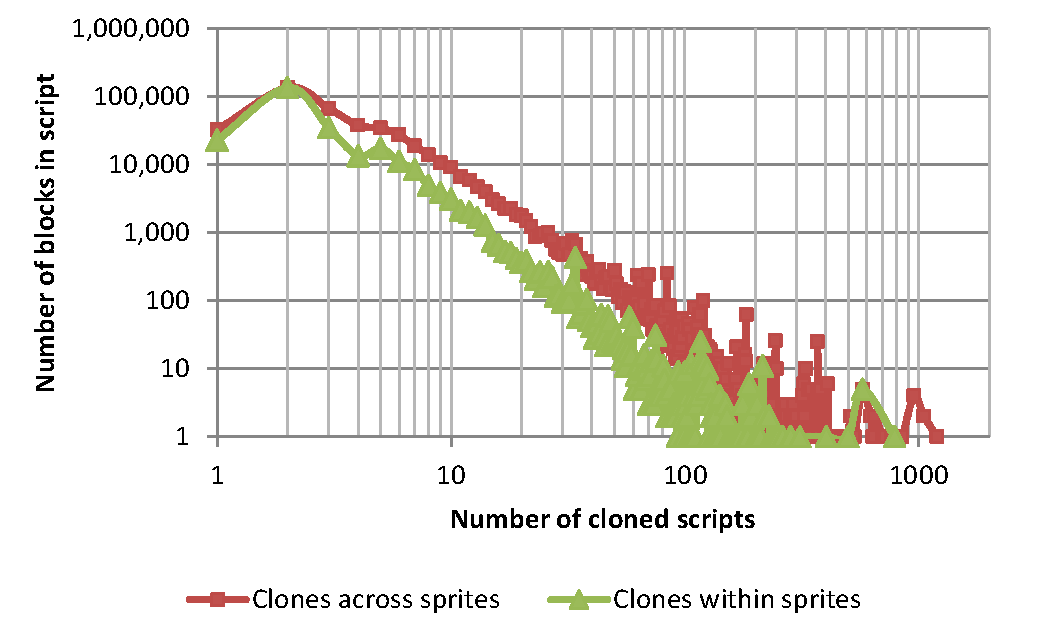
\includegraphics[width=0.45\textwidth]{fig/charts/11cloneslines}
	\caption{Number of cloned scripts of different block sizes across and within sprites}
	\label{fig:cloneslines}
\end{figure}

In total, in the dataset we found 170,532 scripts cloned across sprites in 59,634 (25.54\% of the total non-empty) projects. 726,316 copies of those scripts were found, making each clone being copied an average of 4.26 times. Figure \ref{fig:clonesprojects} plots the distribution of clones across projects. The majority of projects contain up to two cloned scripts; 7.24\% of the projects contain three or more. Figure \ref{fig:clonescopies} plots the number of copies of the identified clones. It is of interest that 79,378 (46.55\%) of the identified clones are copied three or more times, and even in 585 cases from 411 projects they are copied more than 50 times and up to 974 \footnote{\todo{link}}. Manual inspection of the mostly copied clones revealed that they were scripts used multiple times to cater for different parameter values, sometimes in multiple sprites.

\begin{figure}
	\centering
	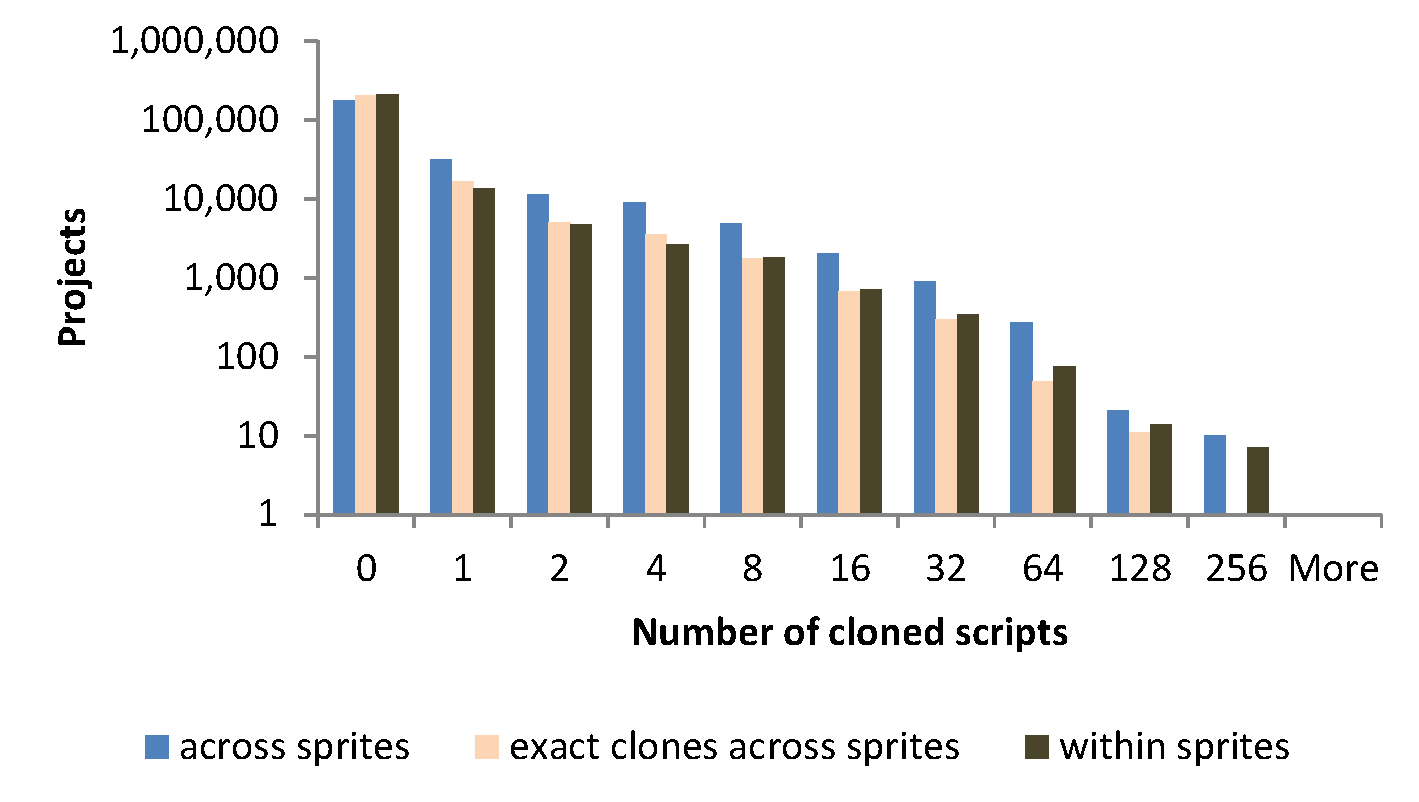
\includegraphics[width=0.45\textwidth]{fig/charts/11clonesprojects}
	\caption{Histogram of the number of cloned scripts found in the dataset projects}
	\label{fig:clonesprojects}
\end{figure}

\begin{figure}
	\centering
	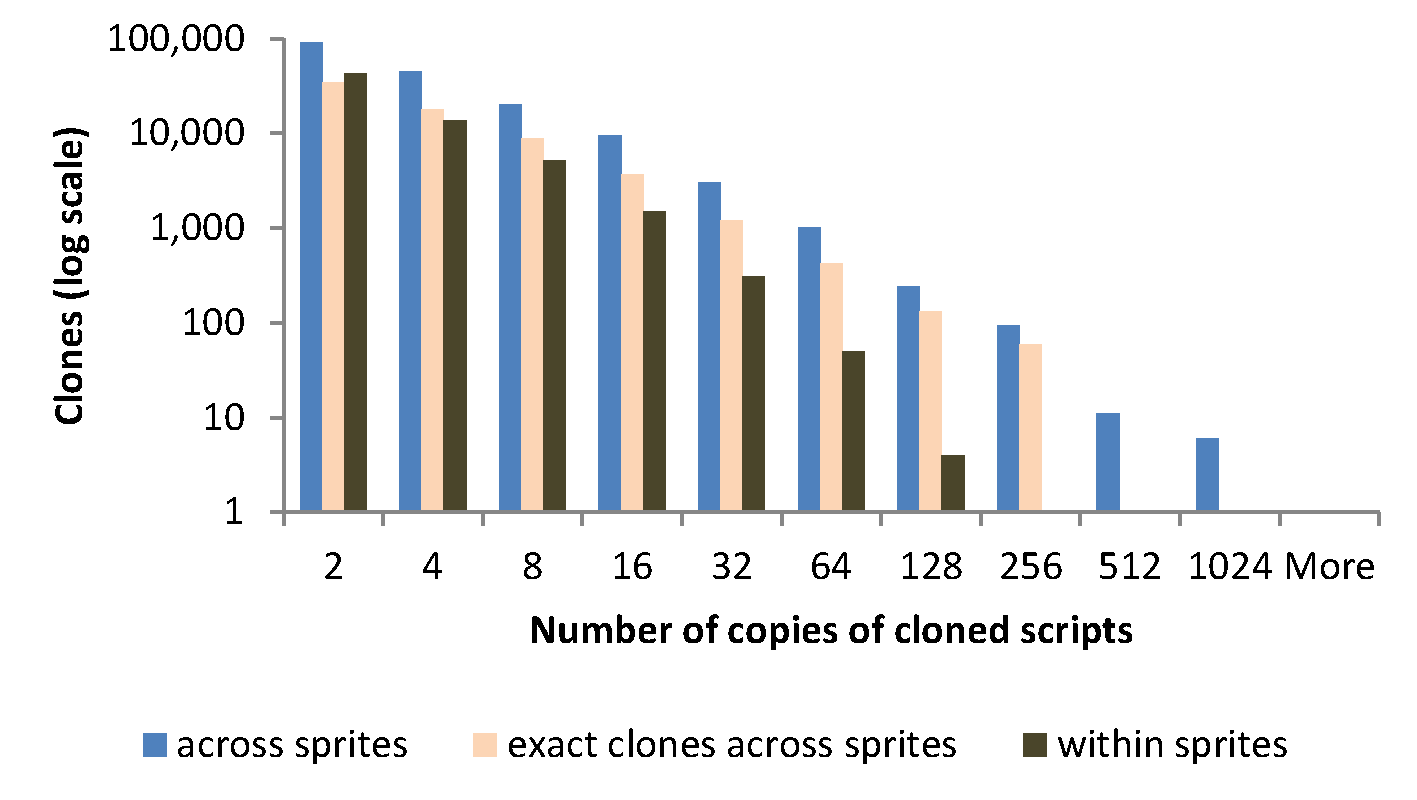
\includegraphics[width=0.45\textwidth]{fig/charts/11clonescopies}
	\caption{Histogram of the number of copies of the identified clones}
	\label{fig:clonescopies}
\end{figure}

We further inspected which of the identified clones were duplicated only within the same sprite: 63,682 (37.34\% of the total) clones, in 10.14\% of the projects. These are duplication smells that could be avoided by using procedures, which in Scratch can only be defined for specific sprites. The lack of support for project-wide procedures could be the cause for procedure clones. These were measured to 12,878 (7.55\% of the total) clones, in 2.12\% of the projects.

Exact clones were found in 11.81\% of the total projects. Their total number was 66,750 (39.14\% of the total) clones. Exact clones in the same sprite are cases of clearly redundant code. These were rare, found in only 0.87\% of the projects.

Apart from whole scripts we also examined cases with only the first block being different. In first block is commonly the event block and, by separating this one from the subsequent functionality blocks, we could examine if programmers assign the same functionality to handle different events. Cloned functionality blocks



dead code -unconnected blocks,
previous section: A significant number of the defined procedures (13,036 or 6.3\%) are not called in the projects.
This lack of wait-receive syncronizations occurs in 18,669 projects (7.99\% of the total non-empty ones).

long method
large class


coding style -naming -functions, sprites, variables
code block positioning - overlapping /visibility


\begin{figure}
	\begin{center}
		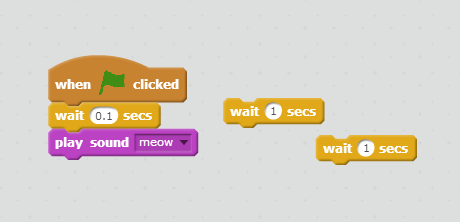
\includegraphics[width=6cm]{fig/Unconnected_clones.png}
		\caption{Cloned blocks that are not connected to an event. Program id: 12237615}
		\label{fig:Unconnected_clones}
	\end{center}
\end{figure} 



Scratch programs are found to be particularly susceptible to the duplicate code smell: code clones were found in one fourth of the projects in the dataset.


\section{Discussion}

\subsection{Implications}
Our results have some interesting implications for designers of educational programming languages. 

\subsubsection{Unconnected Blocks}
In the whole dataset, not just in the programs with clones, we observe unconnected scripts, scripts without an event block and events without associated code. This is a form of \emph{dead code}, code that will never be executed. Because this dead code caused visual clutter, it would be better to have a separate workspace (much like the `backpack in Scratch' where users can store blocks temporarily and use them later. A programming interface could ask actively encourage users to move unconnected block when they exit the environment to encourage a `clean' working space. 

\subsubsection{Code Clones Between Sprites}
With occurrences in one quarter of the 250 thousand programs, the use of exactly identical clones between sprites is extremely common. In a sense, the Scratch users are not to blame here, as Scratch does not support the sharing of procedures between scripts, only within them. So in many cases there is no other way to share the functionality than by making a copy. We are not aware of the underlying rationale of the Scratch team that lead to this decision, however it seems that a large part of the Scratch users would use the functionality to call procedures between sprites.

\subsubsection{Refactoring support for duplicate wait blocks}
In todo{...} of the cases, the programs with duplicate conditions, also signals were present. This means that it is feas

\subsection{Threads to validity}
A thread to validity of this study is the fact that we did not scrap a random sample, but the most recent 250,000 programs. It could be the case that programming habits of Scratch users are changing over time. However, we counterbalanced that by using a very large dataset. Furthermore, for some of the analyses we manually inspected programs \todo{Fenia, which ones?}


\section{Related Work}
\label{sec:related}

\subsection{Code Smells}
Efforts related to our research include works on code smells, initiated by the work by Fowler~\cite{fowler_refactoring:_1999}. His book gives an overview of code smells and corresponding refactorings. Fowler's work was followed by efforts focused on the automatic identification of code smells by means of metrics. Marinescu~\cite{marinescu_detecting_2001} for instance, uses metrics to identify \emph{suspect} classes: classes which could have design flaws. Lanza and Marinescu~\cite{lanza_object-oriented_2006} explain this methodology in more detail. Alves \emph{et al.}~\cite{alves_deriving_2010} focus on a strategy to obtain thresholds for metrics from a benchmark. Olbrich \emph{et al.} furthermore investigates the changes in smells over time, and discusses their impact~\cite{olbrich_evolution_2009}. Moha \emph{et al.}~\cite{moha_decor:_2010} designed the `DECOR' method which automatically generates a smell detection algorithms from specifications. The CCFinder tool~\cite{kamiya_ccfinder:_2002} finally, aims at detecting clones in source code, which are similar to our \dup smell.

\subsection{Smells beyond the OO paradigm}
In recent times, code smells have been applied to programs outside of the regular programming domain. In our past work, we have, for example, studied code smells within spreadsheets, both at the formula level~\cite{hermans_detecting_2014} and between worksheets~\cite{hermans_detecting_2012}.

More recently, we compared two datasets: one containing spreadsheets which users found unmaintainable, and a version of the same spreadsheets rebuilt by professional spreadsheet developers. The results show that the improved versions suffered from smells to a lesser degree, increasing our confidence that presence of smells indeed coincides with users finding spreadsheets hard to maintain~\cite{jansen_code_2015}.

In addition to spreadsheets, code smells have also been studied in the context of Yahoo! Pipes a web mashup tool. An experiment demonstrated that users preferred the non-smelly versions of Yahoo Pipes programs~\cite{stolee_refactoring_2011}. 

%\subsection{Agile practices in education}
%A third related line of work are research directions where other methods from agile development, like testing and refactoring, have been applied in education. For example, the use of test-driven development has been studied within the context of programming education at university level, using text-based languages in several studies. Most controlled experiments resulted in increased code quality for the group of students using TDD, for example [13] reported on a 35\% reduction in defects, while [14] found 45\%. For an extensive overview of TDD approaches in university programming courses, see [15]. \todo{referenties fixen}

\subsection{Quality of Scratch programs}
Finally, there are other works on the quality of Scratch programs. There is for example the Hairball Scratch extension~\cite{boe_hairball:_2013}, which is a lint-like static analysis tool for Scratch that can detect, for example, unmatched broadcast and receive blocks, infinite loops and duplication. An evaluation of 100 Scratch programs showed that Scratch programs indeed suffer from duplication and bad naming~\cite{moreno_automatic_2014}.

Most related to our study is the work by Moreno \emph{et al.}~\cite{moreno-leon_dr._2015} who gave automated feedback on Scratch programs to 100 children aged 10 to 14. Their results demonstrated that feedback on code quality helped improve students' programming skills.


\bibliographystyle{abbrv}
\bibliography{zotero}
\end{document}
